\documentclass[a4paper]{article}

% info progetto
\newcommand{\NST}{Nicola Sgarbossa }
\newcommand{\LDG}{Prof. Luigi De Giovanni}
\newcommand{\DB}{Prof. Davide Bresolin}
\newcommand{\azienda}{Lynx S.p.a.}

% membri del gruppo 
\newcommand{\AS}{Alessandro Sgreva}
\newcommand{\NS}{Nicola Salvadore}

%Lista dei comandi relativi al documento
\newcommand{\docTitle}{Relazione attività di tirocinio}
\newcommand{\annoAcc}{2020-2021}
\newcommand{\red}{\NS{} - 2026882}
\newcommand{\desc}{Breve relazione su tirocinio presso \azienda}
\newcommand{\destinatari}{\DB}



% pacakges
\usepackage{pdflscape}
\usepackage{geometry}
\usepackage{hyperref} %  link
\usepackage{graphicx} %immagini
\usepackage{wrapfig} % immagini wrapped
\usepackage{titlesec} %per creazione di una section personalizzata
\usepackage{float} %per il posizionamento delle figure

\usepackage[shortlabels]{enumitem} % per elenchi personalizzati
\usepackage{titlesec} %per creazione di una section personalizzata

% package per la lingua / caratteri
\usepackage[italian]{babel}
\usepackage[utf8]{inputenc}
\usepackage[T1]{fontenc}
\usepackage{comment}

\usepackage{fancyhdr} % per header e footer
\usepackage{lastpage} % per avere l'indice dell'ultima pagina

\usepackage{tabularx} % tabelle
\usepackage[table]{xcolor} % definizione colore di sfondo per tabelle
\usepackage{longtable} % permette di estendere le tabelle su più pagine

\usepackage{chngcntr} % per numerazione immagini e tabelle

\usepackage[official]{eurosym} %per poter utilizzare il simbolo dell'euro

\usepackage[titletoc]{appendix} % per poter usare le appendici
\usepackage[official]{eurosym} %per poter utilizzare il simbolo dell'euro
\usepackage{float} %posizionamento delle immagini UC

%Per la creazione dei grafici
\usepackage{pgfplots}
\usetikzlibrary{
	pgfplots.dateplot,
}
\pgfplotsset{width=15cm,compat=1.11}
\usepackage{tikz}

% configurazione
% link
\hypersetup{
	colorlinks=true,
	linkcolor=black,
	filecolor=magenta,
	urlcolor=blue,
}

\graphicspath{res/img/}

% intestazione e piè di pagina
\pagestyle{fancy}
% intestazione
\setlength{\headheight}{25pt}
\lhead{ 
\includegraphics[scale=0.3]{./res/img/cropped_logo.png} }
\rhead{ \docTitle{} }
% piè di pagina \\
\renewcommand{\footrulewidth}{0.4pt} % per avere una linea nel footer
\cfoot{}
\rfoot{Pagina \thepage{} di \pageref{LastPage}}

% tabelle
\def\arraystretch{1.5} % padding
% comandi e colori tabelle
\definecolor{lightRowColor}{HTML}{fafafa}
\definecolor{darkRowColor}{HTML}{ffcccb}

\newcommand{\coloredTableHead}{\rowcolor[HTML]{b61827}}
\newcommand{\lightTableRow}{\rowcolor{lightRowColor}}
\newcommand{\darkTableRow}{\rowcolor{darkRowColor}}

% per numerazione immagini e tabelle
% --> la numerazione dipende dalla subsection in cui ci si trova
\counterwithin{table}{subsection}
\counterwithin{figure}{subsection}

% definizione del comando subsubsubsection
\titleclass{\subsubsubsection}{straight}[\subsection]

\newcounter{subsubsubsection}[subsubsection]
\renewcommand\thesubsubsubsection{\thesubsubsection.\arabic{subsubsubsection}}

\titleformat{\subsubsubsection}
  {\normalfont\normalsize\bfseries}{\thesubsubsubsection}{1em}{}
\titlespacing*{\subsubsubsection}
{0pt}{3.25ex plus 1ex minus .2ex}{1.5ex plus .2ex}

\makeatletter
\def\toclevel@subsubsubsection{4}
\def\toclevel@paragraph{5}
\def\toclevel@paragraph{6}
\def\l@subsubsubsection{\@dottedtocline{4}{7em}{4em}}
\def\l@paragraph{\@dottedtocline{5}{10em}{5em}}
\def\l@subparagraph{\@dottedtocline{6}{14em}{6em}}
\makeatother

\setcounter{secnumdepth}{4}
\setcounter{tocdepth}{4}


\begin{document}
	 % numerazione delle tabelle dipendente dalla section ( e non dalla subsection)
	 \counterwithin{table}{section}
	 
	 % copertina
	 \thispagestyle{empty}
\begin{titlepage}
	\begin{center}
		\vfill
        \large
		
\includegraphics[scale=0.35]{./res/img/logo_short.png}
		\vfill
		\begin{Huge}
			\textbf{\docTitle}
		\end{Huge}
		\vfill
		\vspace*{\fill}
		\begin{tabular}{r|l}
			\textbf{Studente} & \red \\
			\textbf{Destinato a} & \destinatari \\
			\textbf{Tutor universitario} & \LDG \\
			\textbf{Tutor aziendale} & \NST \\
			\textbf{Anno accademico} & \annoAcc \\
		\end{tabular}	
		\normalsize
		\vfill
		\textbf{Descrizione}\\
		\textit{\desc} \\
		\vfill
	\end{center}
\end{titlepage}

	 
	 % indice
	 \renewcommand*\contentsname{Sommario}
	 \tableofcontents
	 \pagebreak

	 % informazioni generali
	 \section{Introduzione}

\subsection{L'azienda}
Il Gruppo Lynx è una realtà internazionale che opera nell'ambito della consulenza informatica. La consolidata expertise maturata in ambito tecnologico e di business, unitamente all'utilizzo di collaudate metodologie gestionali, consente a Lynx di proporsi ai propri Clienti come partner strategico per la realizzazione di progetti innovativi con soluzioni e know-how specifici. \\
Obiettivo principale di Lynx è continuare ad accrescere le proprie competenze funzionali e tecnologiche nei settori in cui opera, per offrire soluzioni efficaci che rispondano alle esigenze dei clienti. \\
Lynx è attiva in molti settori a livello internazionale, in particolare in quello dei servizi informatici nell'ambito della finanza, ma anche nel settore energetico e dei trasporti. \\

\begin{figure}[!ht]
	\centering
	
\includegraphics[width=0.6\textwidth]{./res/img/settori.png}
	\caption{Percentuali di aziende servite da Lynx nei vari settori.}
\end{figure}

\subsection{Intesa SanPaolo e Sportello}
\azienda collabora da anni con Intesa SanPaolo l'istituto bancario più grande del paese che conta moltissimi dipendenti. Tra i servizi offerti c'è l'applicazione che gestisce il workflow e i servizi all'interno delle filiali, denominata \textbf{Sportello}. \\
Lynx in collaborazione con Microsoft è stata chiamata a gestire il progetto di \textbf{Nuovo Sportello}. L'applicativo opera in tutte le filiali Intesa SanPaolo presenti sul territorio nazionale ed è utilizzato ogni giorno da migliaia di utenti. \\
Lynx offre a Intesa SanPaolo per Nuovo Sportello un servizio di AM (Assets Management) e uno di Evolutiva per lo sviluppo di nuove funzionalità. \\
La parte client del Nuovo Sportello è una web application basata su framework ASP.NET, utilizzabile su browser. Questo rende l'applicazione di facile utilizzo, versatile e molto più facile da mantenere. \\ 
In una sezione successiva descriverò in dettaglio la struttura e l'architettura del software. \\

\subsection{Ruoli e organizzazione aziendale}
Essendo Lynx una realtà molto estesa che conta molti dipendenti, durante il tirocinio sono riuscito a venire a contatto con poche persone, ma ho potuto farmi un'idea generale della sua organizzazione. Ogni macro-progetto con un cliente specificato, come ad esempio Sportello, è seguito da un buon numero di persone divise in team. Per quanto riguarda Sportello, si seguono molto i principi del modello Agile:
\begin{itemize}
	\item Soddisfazione del cliente, attraverso un consegna continua di software validato.
	\item Continuous Delivery (nel caso di sportello avviene un rilascio major ogni mese, che contiene bugfixing e nuove funzionalità)
	\item Continua iterazione e coperazione tra cliente, azienda e sviluppatori.
	\item Iterazione di tipo faccia a faccia tra persone.
	\item Ritmo sostenibile di sviluppo.
	\item Attenzione alla qualità del codice e al buon design.
\end{itemize}
Ho notato anche affinità con i principi del framework SCRUM, nella divisione in team, l'iterazione quotidiana e le scadenze.\\
Durante la mia esperienza di tirocinio ho avuto modo di far parte di due team diversi e vedere in generale il metodo di lavoro aziendale. 

\subsubsection{Gestione del telelavoro}
Durante la pandemia come moltissime altre aziende, Lynx ha aumentato il numero di ore e persone in telelavoro. Anche agli stagisti è capitata la stessa sorte. Tuttavia ho potuto constatare che il lavoro è ben organizzato, grazie alla lunga esperienza di Lynx nel settore.
La maggior parte del lavoro l'ho svolto da casa, con gli strumenti adatti. Ho potuto però notare la mancanza dell'iterazione fisica importante anche nel nostro settore, nel quale è fondamentale stringere relazioni.

\pagebreak	 
	 \pagebreak

	 \section{Nuovo Sportello}

In questa sezione descriverò in modo dettagliato le parti dell'infrastruttura che ho esplorato durante il tirocinio e che ho approfondito grazie al lavoro svolto.

\subsection{Formazione e descrizione di Nuovo Sportello}

Nel primo periodo c'è stato naturalmente un periodo di formazione, svolto in presenza nella sede di Padova di Lynx. \\ 
pdfDurante le ore di formazione, il tutor \NST mi ha presentato l'architettura di Sportello in ogni sua parte, con le tecnologie utilizzate. Ho avuto modo di entrare in contatto per la prima volta con un sistema molto complesso e di vederne la sua evoluzione nel tempo. \\

\begin{figure}[!ht]
    \centering
	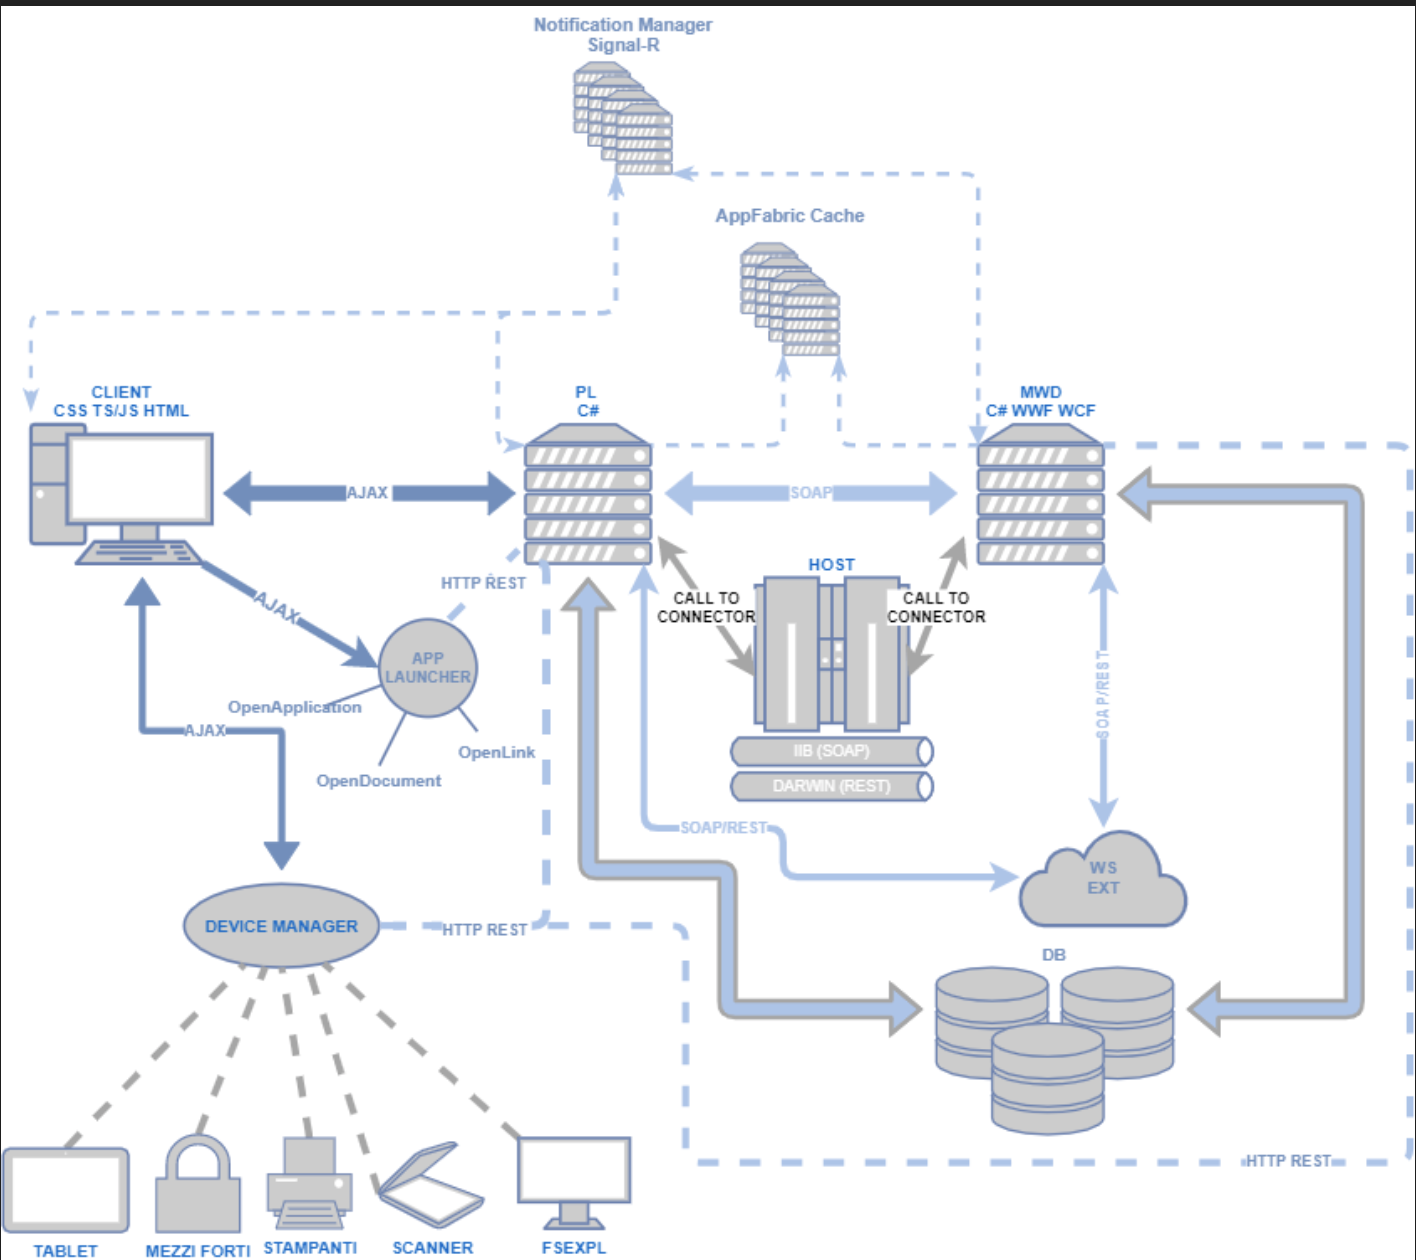
\includegraphics[width=0.85\textwidth]{./res/img/infrastruttura sportello.png}
    \caption{Overview dell'infrastruttura di Sportello}
\end{figure}

Com'è possibile vedere dalla figura la parte front-end dell'infrastruttura a sinistra è basata su ASP.NET. Il client scritto in Typescript e HTML comunica tramite chiamate Ajax con un server chiamato Presentation Layer scritto in C\#, il quale contiene tutta la logica complessa e ha la possibilità di eseguire chiamate ai server di Intesa SanPaolo o a collegarsi a servizi Middleware. Questa parte è responsabile anche del collegamento a device fisici controllabili via software. \\
Nel back-end ho già nominato i server Middleware che si occupano di esporre servizi basati su protocolli di tipo SOAP. In questo frangente sono venuto a contatto con una tecnologia Microsoft: \textit{WCF}. Windows Communication Foundation (WCF) è un framework per costruire servizi in modo sicuro ed è efficiente. È utilizzata anche una versione Event Driven con una programmazione grafica, attraverso file .xaml, chiamata Windows Workflow Foundation. \\
Sempre a back-end sono disponibili tutti i DB basati su Microsoft SQL Server e l'host di Intesa SanPaolo, server contente tutti i dati della banca. \\

\subsubsection{ASP.NET}
ASP.NET è un framework creato da Microsoft per lo sviluppo di web application. Segue il pattern MVC (Model View Controller), ripreso poi dall'infrastruttura front end di Sportello. La view è costruita attraverso le normali tecnologie web, mentre il model e il controller sono scritti in C\#. I model non sono nient'altro che \textit{contract} che vengono utilizzati nel comunicazioni Ajax tra le componenti. I controller espongono metodi utili al front end implementandone la logica di fondo.  

\subsubsection{SOAP}
Durante la prima fase del tirocinio mi è stato molto utile il concetto di chiamata SOAP. Il \textit{Simple Object Access Protocol} è utilizzato per scambiare informazioni strutturate basato principalmente su HTTP. SOAP utilizza un sistema di incapsulamento delle informazioni e anche per questo è portato per il trasporto di oggetti.

\subsection{Ambienti di Sportello}

Sportello viene sviluppato testato e rilasciato in 3 ambienti diversi, chiamati: \textbf{SVIL}, \textbf{UAT} e \textbf{SYSTEM}.

\subsubsection{SVIL}

L'ambiente di sviluppo é il primo in cui vengono rilasciate le modifiche a Sportello. Qui gli sviluppatori su richiesta possono chiedere una build (tramite RTC, il sistema di versioning utilizzato) e testare l'applicazione eseguendo debugging da browser, per esempio. Come visibile in figura é facile notare che le stesse componenti dell'infrastruttura di sportallo sono replicate all'interno dell'ambiente. Si può notare che SVIL possiede un proprio DB che mantiene anche le proprie configurazioni, oltre ad avere accesso ai database di SYSTEM, in produzione. \\
É presente in realtà un altro ambiente utilizzato soprattutto in per interventi per ticket con altra priorità. Questo ambiente chiamato \textbf{BFIX} é mantenuto sempre allineato con SYSTEM, in modo tale da risolvere problemi importanti che sono presenti in produzione e rilasciarli il più velocemente possibile. 


\begin{figure}[!ht]
    \centering
	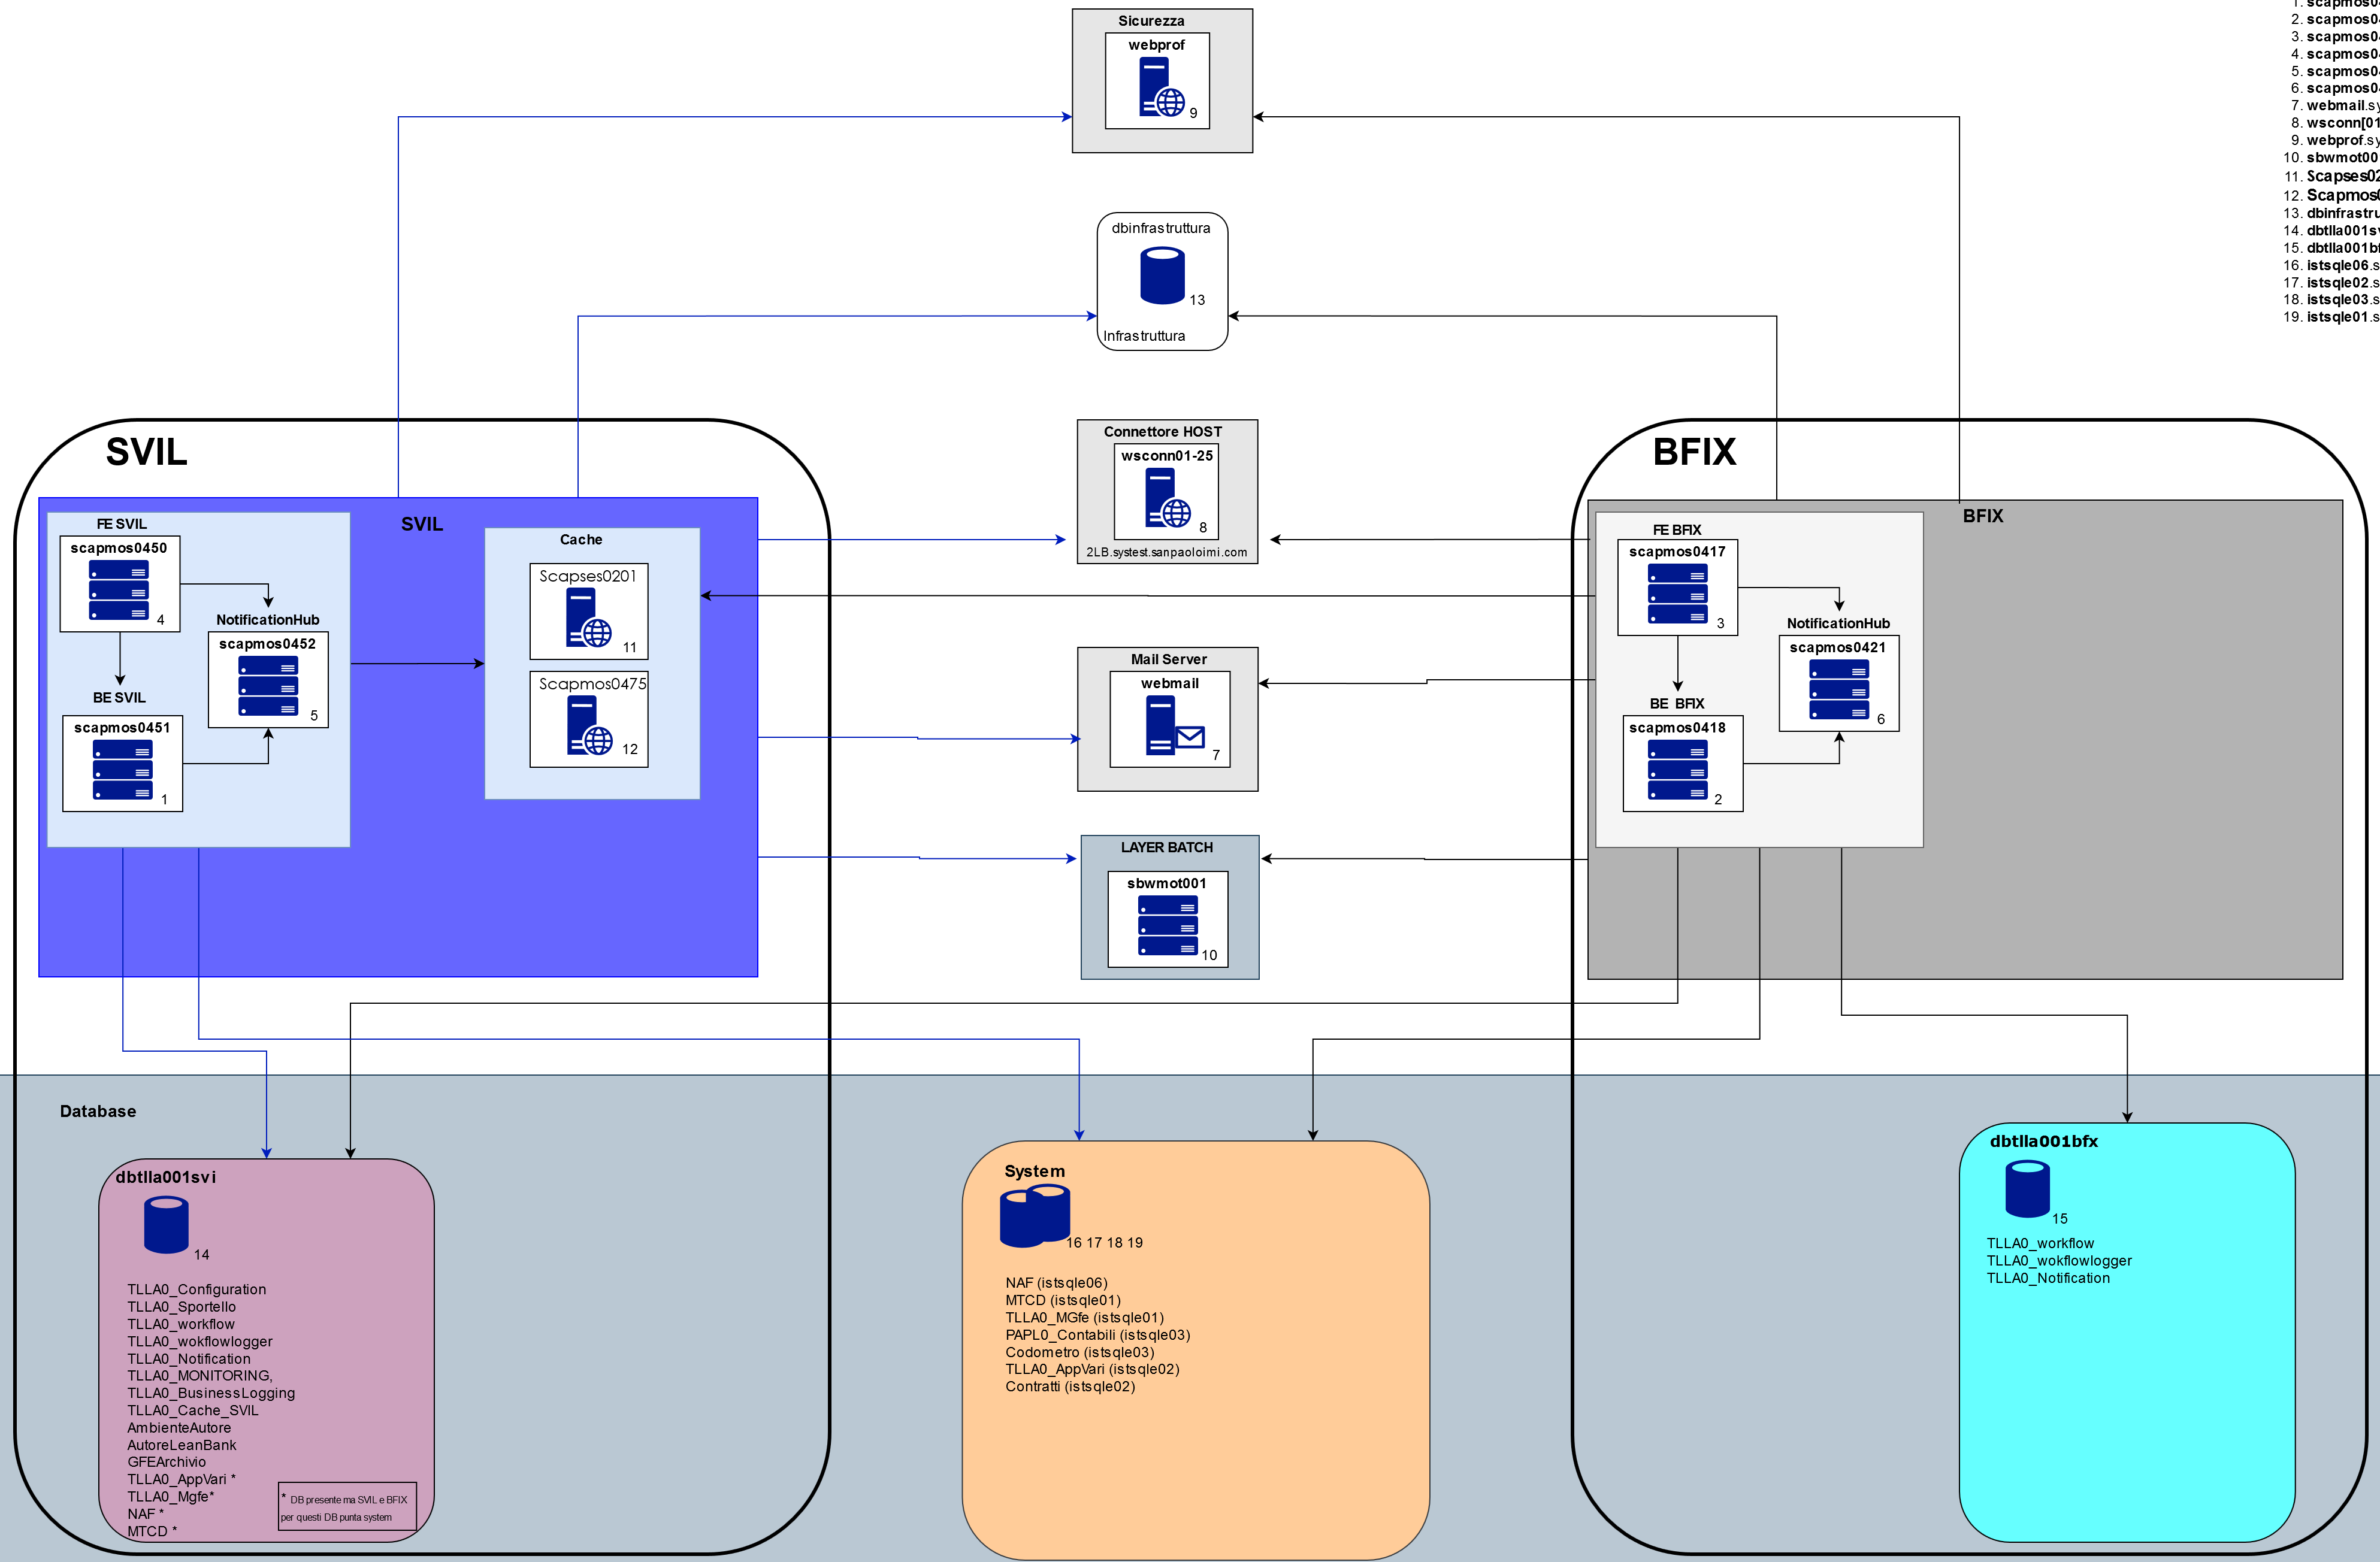
\includegraphics[width=0.85\textwidth]{./res/img/svil-diag.png}
    \caption{Overview dell'infrastruttura dell'ambiente SVIL}
\end{figure}

\subsubsection{UAT}

L'ambiente UAT é predisposto per il testing da parte di un team predisposto dal cliente. Qui alcuni dipendenti predisposti di Intesa testano le modifiche più importanti o il rilascio di nuove funzionalità. Su UAT si trova una versione successiva rispetto a quella presente in produzione. Se il software passa i requisiti imposti dal cliente, può essere rilasciato in SYSTEM.

\begin{comment}
\begin{figure}[!ht]
    \centering
	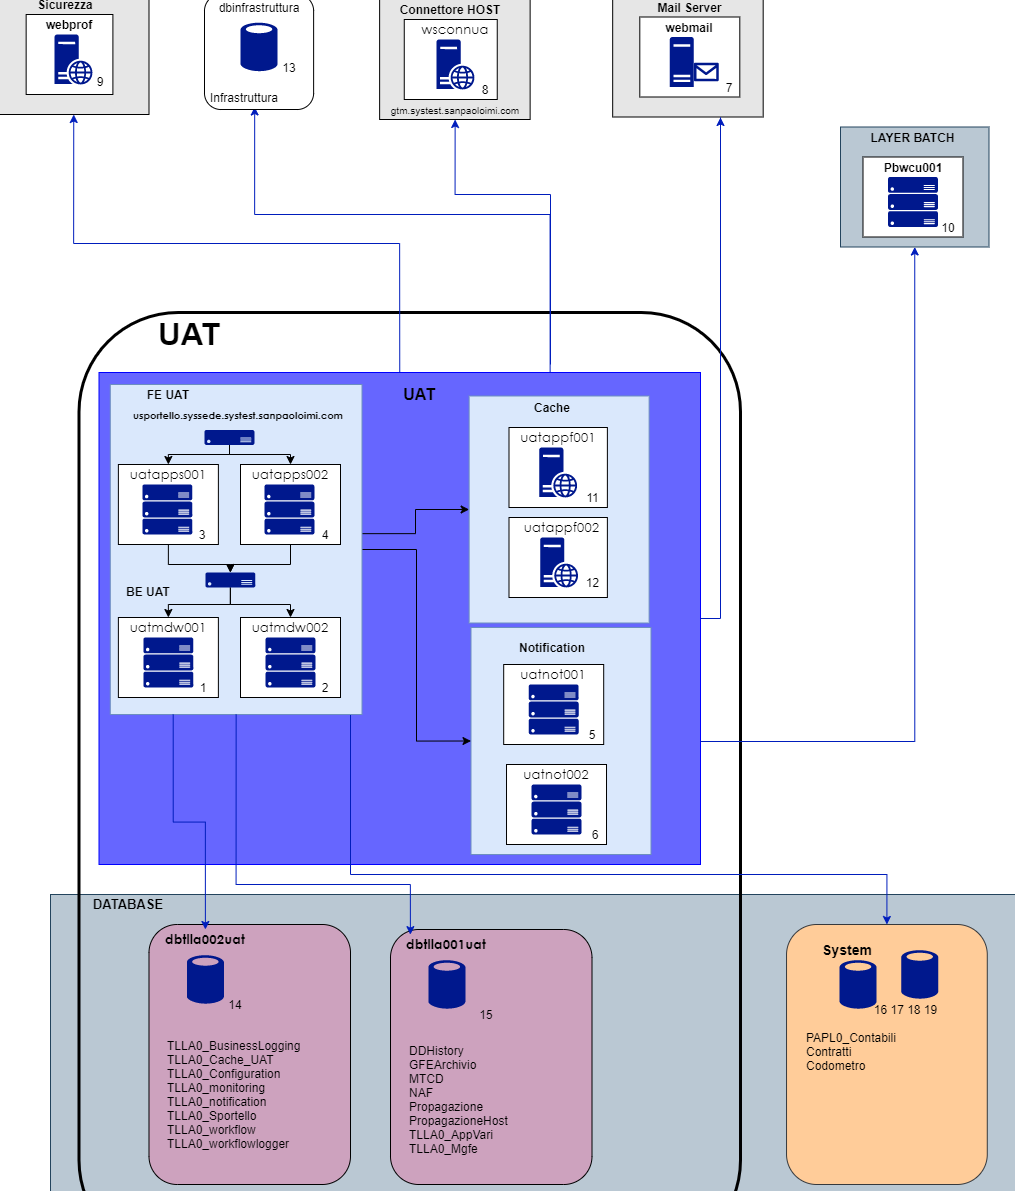
\includegraphics[width=0.75\textwidth]{./res/img/Collegamenti_UAT.png}
    \caption{Overview dell'infrastruttura dell'ambiente UAT}
\end{figure}
\end{comment}

\subsubsection{SYSTEM}

SYSTEM é l'ambiente di produzione. Qui esiste solo codice verificato e testato. Inoltre il sistema é costantemente monitorato sia dal cliente che da Lynx stessa.  \\
Si può notare dallo schema che i server stessi sono localizzati in punti geografici diversi, ma hanno lo stesso punto di accesso e gli stessi collegamenti alle altre componenti.  

\begin{figure}[!ht]
    \centering
	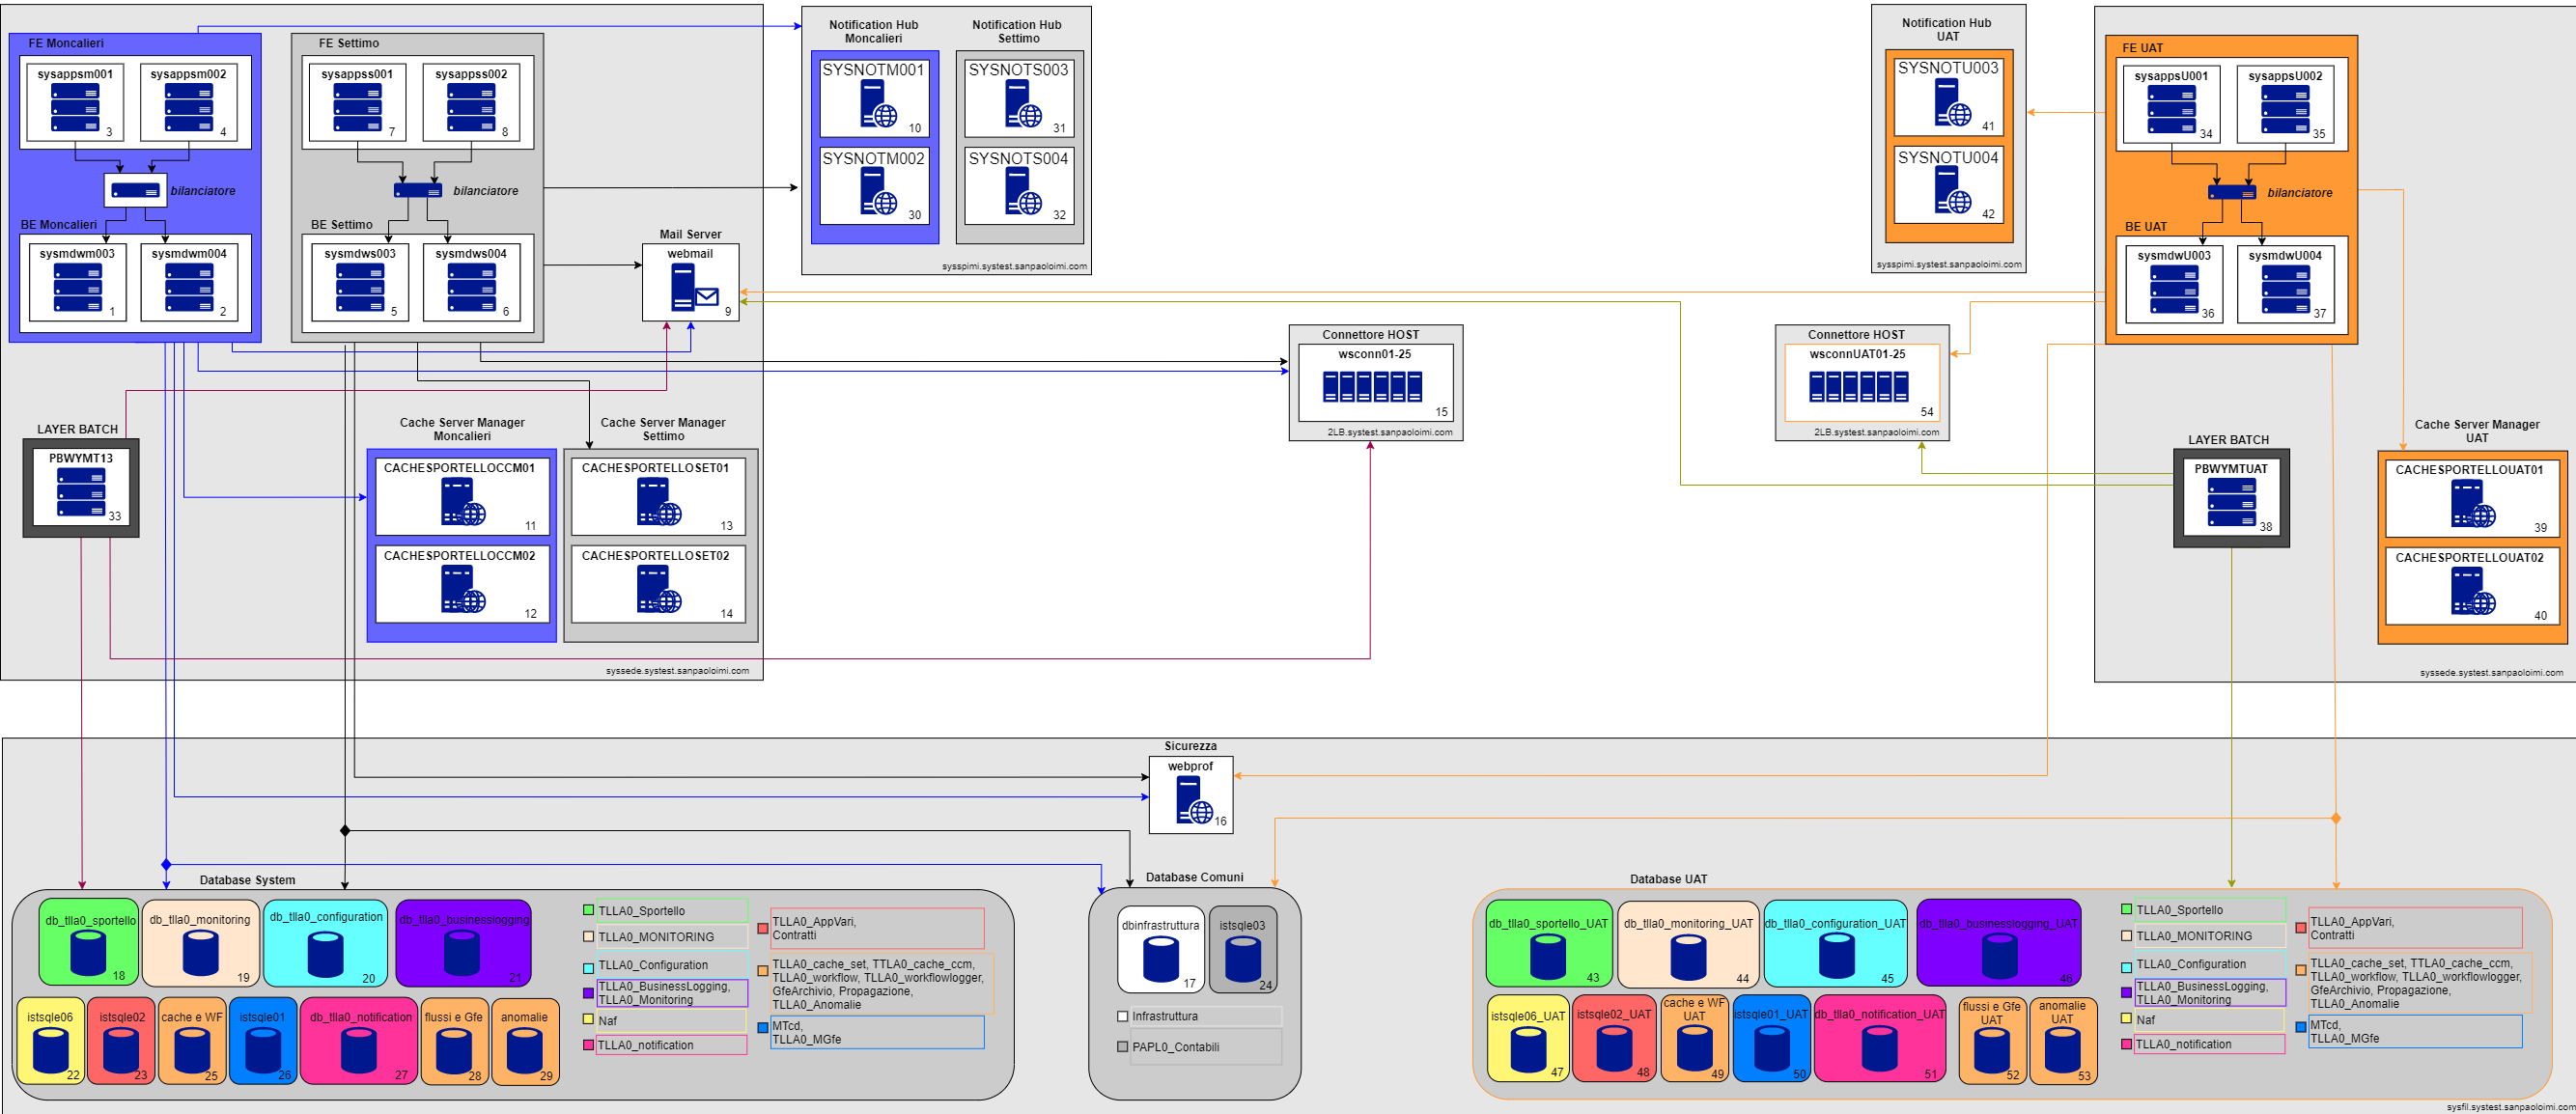
\includegraphics[width=0.85\textwidth]{./res/img/SchemiAmbienti_SYSTEM-UAT_v1.1.png}
    \caption{Overview dell'infrastruttura dell'ambiente SYSTEM e UAT}
\end{figure}

\subsection{Strumenti utilizzati}

\subsubsection{Visual Studio 2013/2017}
\begin{wrapfigure}{R}{0.25\textwidth}
    \begin{center}
        
\includegraphics[width=0.15\textwidth]{./res/img/visual-studio-2013-logo.png}
        \caption{Logo di Visual Studio}
    \end{center}
\end{wrapfigure}

L'IDE principale utilizzato durante lo sviluppo é stato naturalmente Visual Studio. Integrato nativamente con il framework ASP.NET e il linguaggio C\#, non é stato di difficile utilizzo. \\ É disponibile un interfaccia per la gestione dei pacchetti e delle librerie esterne tramite \textbf{NuGet}. É stato interessante gestire e integrare le varie \textbf{.dll} (estensione delle librerie Windows). \\ É ovviamente presente uno strumento per la build automatica e uno per il testing. \\
Vengono utilizzate altre versioni di Visual Studio (Microsoft SQL Server Management o VS 2017) per la gestione e l'interrogazione dei database.

\subsubsection{Rational Team Concert (RTC)}

\begin{wrapfigure}{R}{0.25\textwidth}
    \begin{center}
        
\includegraphics[width=0.25\textwidth]{./res/img/1-IBM-rational-1.png}
        \caption{Logo di IBM RTC}
    \end{center}
\end{wrapfigure}

\textbf{RTC} é il \textit{version control system} sviluppato da IBM. Essendo abituato ad altri tipi di sistemi basati su \textbf{Git} é stato per me uno scoglio abituarmi, dato che l'applicazione, come anche i miei colleghi, utilizzano terminologia diversa. Dove su Git si utilizzano i \textit{branch} su RTC si utilizzano gli \textit{stream}, ad esempio. Oltre ad essere diverso a livello di terminologia, lo é anche a livello di complessità e di funzionalità offerte. É possibile, ad esempio, scaricare parte della \textit{repository}, lavorare solo su parte di essa o sincronizzarla parzialmente. Ha una buona gestione dei team e si può integrare con le build dell'intera applicazione in modo tale da automatizzarla. Inoltre, riesce a gestire i tre ambienti di Sportello, caricandosi del deploy di gran parte delle sue componenti. 

\subsubsection{Browser}
Lato client Nuovo Sportello é una web application ed é quindi accessibile tramite browser. É nativamente supportata da \textit{Internet Explorer}, ma é da tempo in corso un porting di alcune funzionalità anche su \textit{Google Chrome} e \textit{Mozilla Firefox}. \\
Il test su browser, soprattutto tramite debugger integrato si é rivelato molto utile durante la prima fase di interazione con il cliente. 

\subsubsection{Sonarqube}
Sonarqube permette l'analisi sia statica che dinamica del codice, tramite un'interfaccia semplice e pratica. L'ho utilizzato soprattutto per misurare il code coverage durante la scrittura delle funzioni di test. 

\subsubsection{Citrix}
Citrix é uno strumento che permette di accedere alle macchine virtuali, sulle quali sono installati tutti gli strumenti per lavorare su Sportello. 

\subsubsection{RedMine}
Redmine é un portale utilizzato da Lynx per tenere tutta la documentazione di ogni progetto. Da questa o attinto per la maggior parte delle informazioni tecniche riguardanti Sportello.

\subsubsection{Comunicazione}
Per la comunicazione ci sono diversi canali. Lynx e Intesa utilizzano \textit{Microsoft Teams} per le chat di gruppo e tra dipendenti. Per le comunicazioni ufficiali via mail si utilizza \textit{Outlook}. É stato interessante in questo frangente osservare una transizione di tecnologia, dato che nel periodo del mio tirocinio, Lynx si é spostata da \textit{Skype} a \textit{Microsoft Teams}.

	 \pagebreak

	 \section{Progetto e attività}

Durante il tirocinio ho avuto modo di seguire due commesse con due team differenti. In questa sezione descriverò in dettaglio ciò che ho fatto e in che modalità.

\subsection{PACDI}

PACDI é una nuova funzionalità richiesta dal cliente Intesa SanPaolo. Per svilupparla ho fatto parte di un team di evolutiva. 

\subsubsection{Funzionalità e dettagli}
Dal punto di vista del cliente sportello é formato da un insieme di funzionalità, con sigle univoche di cinque lettere. D'ora in poi in questo documento, le sigle di cinque lettere scritte in maiuscolo (come PACDI) indicano le funzioni messe a disposizione da Sportello. 
Sportello attualmente possiede \textbf{x} funzioni a disposizione. \\
 

	 \pagebreak

	 \section{Conclusioni}

In questa sezione esporrò alcune delle mie considerazioni finali sul tirocinio.

\subsection{Metodologie e workflow}
Durante il tirocinio ho potuto testare il telelavoro. Da una parte credo che mi abbia penalizzato, dall'altra invece aiutato. A parte il periodo iniziale di formazione in ufficio, la maggior parte delle ore lavorative le ho passate a casa. La penalizzazione viene dalle poche relazioni strette con i colleghi. Ho avuto modo di conoscere poche persone e non sempre mi è risultato chiaro il ruolo di tutti o la struttura della gerarchia aziendale. Per forze di causa maggiore non è stato possibile lavorare in ufficio, ma questo è stato sicuramente un fattore di comodità. Ho potuto apprezzare il poter utilizzare il mio hardware e guadagnare il tempo dovuto agli spostamenti. \\
Dal punto di vista dell'organizzazione del lavoro e dei team ho avuto il piacere di collaborare con una azienda seria, che si preoccupa di creare un ambiente lavorativo produttivo. \\
Per quanto riguarda le metodologie, ho notato che vengono utilizzate le più comuni e moderne, come alcuni concetti di Agile e SCRUM, ma non sono ufficializzate in nessun documento o insieme di norme. 
Tuttavia ho potuto toccare anche con mano un'insieme di best practice studiate, ma mai applicate. 

\subsection{Tecnologie utilizzate}
Un aspetto che mi ha leggermente deluso sono state le tecnologie utilizzate durante il tirocinio, spesso datate o atipiche. Mi aspettavo di trovare e utilizzare software all'avanguardia. Mi sono presto ricreduto. Infatti, ho notato subito di quante risorse siano necessarie a un aggiornamento su infrastrutture grandi e controllate come quella di \textit{Sportello}. Ad esempio, utilizzare un IDE diverso più aggiornato di Visual Studio 2013 probabilmente richiederebbe dei cambiamenti, anche a livello di infrastruttura, che i benefici non basterebbero a pareggiare con le risorse utilizzate. Questo esempio si può estendere alle librerie, che richiderebbero mesi per essere sostituite per ottenere miglioramenti minimi. \\ Per non parlare del fattore sicurezza. Essendo Sportello un software bancario, come caratteristica principale deve avere la sicurezza. Utilizzare librerie o software non approvati o non testati in maniera approfondita, non é possibile in un settore del genere. \\
Tuttavia ho visto che Sportello rimane un'infrastruttura dinamica in continuo cambiamento e aggiornamento, che cerca sempre di inseguire la miglior configurazione possibile. Sempre secondo la filosofia: "se funziona quanto basta, non toccare che si guasta", imparata all'università.

\subsection{Conoscenze acquisite}
Oltre ad aver utilizzato un gran numero di tecnologie e strumenti, da me ancora inesplorati, ho imparato a lavorare in un organizzazione strutturata. La divisione in team e la collaborazione, erano esperienze che non avevo ancora provato, nemmeno in altri stage precedenti. Ho avuto modo anche di elaborare un metodo di lavoro adatto ad approciarmi a grossi sistemi, con un grado di complessità elevato.
	 
\end{document}
